\documentclass[11pt,a4paper]{article}

\usepackage[margin=1in]{geometry}
\usepackage[T1]{fontenc}
\usepackage[utf8]{inputenc}
\usepackage{lmodern}
\usepackage{graphicx}
\usepackage{amsmath}
\usepackage{booktabs}
\usepackage{array}
\usepackage{float}
\usepackage{hyperref}
\usepackage{titlesec}
\usepackage{subcaption}

\setcounter{secnumdepth}{3}

\titleformat{\section}{\large\bfseries}{\thesection.}{0.5em}{}
\titleformat{\subsection}{\normalsize\bfseries}{\thesubsection.}{0.5em}{}
\titleformat{\subsubsection}{\normalsize\bfseries}{\thesubsubsection.}{0.5em}{}

\title{Interpreting Earth Observation Events using Symbolic Multi-Agent Systems and Natural Language Generation}
\author{Stefano Infusini \\ \href{mailto:s5211120@studenti.unige.it}{s5211120@studenti.unige.it}}
\date{15 April 2026}

\begin{document}

\maketitle

\vspace{1cm}

\section*{Details of the Proposal}

\subsection*{1.1 Full Specification of the Proposal}

The project consists in the usage of a symbolic multi-agent system for monitoring environmental changes using satellite-derived Earth Observation (EO) indicators. The project integrates techniques from Symbolic and Distributed Artificial Intelligence (S\&DAI) and Natural Language Processing (NLP), with the goal of demonstrating how symbolic reasoning and language technologies can be combined to interpret EO data in a transparent and structured way.

The workflow of the project is divided into three conceptual levels.

The first level is the EO level, where a small dataset of satellite-derived EO indicators is defined. In the current implementation, these indicators are extracted directly from Sentinel-2 satellite imagery for a limited number of wildfire and flood events. The extracted indicators include values such as vegetation loss percentage, burned area percentage, and water increase percentage.

The second level is a symbolic multi-agent architecture implemented in Jason. The system includes three agent types: a ForestAgent responsible for reasoning about vegetation-related indicators, a WaterAgent responsible for reasoning about water-related indicators, and a CoordinatorAgent responsible for collecting the conclusions produced by the other agents and coordinating the final output.

The third level is the NLP layer, implemented in Python, which transforms the symbolic conclusions produced by the agents into human-readable natural language explanations using template-based Natural Language Generation supported by a small ontology representing environmental concepts such as events, locations, and causes.

\subsection*{1.2 The Kind of the Proposal}

This project is a creative proposal.

\subsection*{1.3 The Range of Points / Difficulty of the Proposal}

The project is classified as hard since it requires the integration of EO processing, symbolic multi-agent reasoning, and natural language generation.

\newpage

\section{Introduction}

Earth Observation data provide a powerful tool for monitoring environmental changes such as floods and wildfires. Satellite imagery can reveal variations in vegetation health, burned areas, and water extent across large geographic regions. However, interpreting these data in a transparent and explainable way remains challenging.

The project presented in this report explores the integration of satellite-derived environmental indicators with symbolic multi-agent reasoning and Natural Language Processing techniques. Instead of treating EO indicators only as numerical outputs, the system interprets them through logical reasoning performed by specialized agents and communicates the conclusions through natural language explanations.

The overall objective is to build a prototype system capable of transforming Earth Observation evidence into structured interpretations that remain transparent and explainable.

\section{Project Architecture}

The system is organized into three conceptual layers.

The first layer is the \textbf{EO layer}, responsible for extracting environmental indicators from satellite imagery. These indicators represent measurable environmental changes such as vegetation loss or water increase.

The second layer is a \textbf{symbolic multi-agent system} implemented in Jason. In this layer, agents maintain belief bases containing EO indicators and apply logical rules to infer environmental events. Three agent types are considered: a ForestAgent responsible for vegetation-related reasoning, a WaterAgent responsible for water-related reasoning, and a CoordinatorAgent responsible for collecting the conclusions produced by the other agents.

The third layer is the \textbf{Natural Language Processing layer}. This module transforms the symbolic conclusions produced by the agents into human-readable explanations using template-based Natural Language Generation supported by a small ontology.

The current implementation focuses on the first layer, which extracts EO indicators from satellite imagery.

\section{EO Data Processing}

The EO layer is based on a small dataset of representative environmental events derived from Sentinel-2 imagery. In the current implementation, six events were selected: three wildfire events and three flood events. For each event, one image acquired before the event and one image acquired after the event were used in order to compute change-based indicators.

\subsection{Dataset}

The dataset used in this project consists of the following events:

\begin{itemize}
\item Wildfire in Greece
\item Wildfire in Turkey
\item Wildfire in Serra da Estrela (Portugal)
\item Flood in Emilia-Romagna (Italy)
\item Flood in Ahr Valley (Germany)
\item Flood in Pakistan
\end{itemize}

The data were organized using the following structure:

\begin{verbatim}
Wildfires_data/
   Greece/
      before_wildfire/
      after_wildfire/
   Turkey/
      before_wildfire/
      after_wildfire/
   SerraDaEstrela/
      before_wildfire/
      after_wildfire/

Flooding_data/
   Emilia/
      before_flooding/
      after_flooding/
   Ahr_valley/
      before_flooding/
      after_flooding/
   Pakistan/
      before_flooding/
      after_flooding/
\end{verbatim}

\subsection{Sentinel-2 Data and Bands}

The analysis uses Sentinel-2 Level-2A imagery. The following spectral bands were used:

\begin{itemize}
\item B03 (Green)
\item B04 (Red)
\item B08 (Near Infrared)
\item B12 (Short-Wave Infrared)
\end{itemize}

These bands allow the computation of spectral indices commonly used for vegetation monitoring, burn detection, and water detection.

\subsection{Processing Workflow}

Two Python notebooks were developed to automate the EO preprocessing stage:

\begin{itemize}
\item \texttt{wildfire\_eo\_indicators.ipynb}
\item \texttt{flood\_eo\_indicators.ipynb}
\end{itemize}

The workflow implemented in these notebooks consists of the following steps:

\begin{enumerate}
\item loading the required GeoTIFF bands
\item converting raster arrays to floating-point values
\item creating a valid-pixel mask
\item computing spectral indices
\item deriving binary masks
\item computing summary statistics
\item exporting the results to CSV tables
\end{enumerate}

\subsection{Wildfire Indicators}

Wildfire analysis was based on the computation of NDVI, NBR, and dNBR.

\subsubsection{Normalized Difference Vegetation Index}

\begin{equation}
NDVI = \frac{B08 - B04}{B08 + B04}
\end{equation}

NDVI measures vegetation condition. Lower NDVI values after an event indicate vegetation damage.

\subsubsection{Normalized Burn Ratio}

\begin{equation}
NBR = \frac{B08 - B12}{B08 + B12}
\end{equation}

Burn severity is estimated using:

\begin{equation}
dNBR = NBR_{before} - NBR_{after}
\end{equation}

Pixels above a selected threshold are classified as burned.

\subsection{Flood Indicators}

Flood analysis was based on the Normalized Difference Water Index.

\begin{equation}
NDWI = \frac{B03 - B08}{B03 + B08}
\end{equation}

NDWI allows the detection of water surfaces and the creation of water masks. Newly flooded areas are detected by comparing water masks before and after the event.

\subsection{Results}

\subsubsection{Flood Results}

\begin{table}[H]
\centering
\caption{Flood indicators derived from Sentinel-2 imagery}
\begin{tabular}{lcccc}
\toprule
Event & NDWI before & NDWI after & Water increase (\%) & New flood (\%) \\
\midrule
Ahr Valley & -0.5759 & -0.7076 & 0.1556 & 0.1620 \\
Emilia & -0.5065 & -0.3007 & 22.7252 & 22.8971 \\
Pakistan & -0.2072 & 0.0037 & 40.5222 & 42.7007 \\
\bottomrule
\end{tabular}
\end{table}

For floods, Emilia-Romagna and Pakistan present strong flood signals with large increases in water-covered area. In particular, the Pakistan flood shows an extensive expansion of water across the floodplain. In contrast, the Ahr Valley flood produces a much smaller increase in detected water area because the flooding occurred mainly along a narrow river corridor. For the Ahr Valley case, the post-event image was acquired on 21 July 2021, several days after the flood peak of 14--15 July 2021. As a result, the extracted flood signal is likely weaker than the actual maximum flood extent. Following we present the Emilia-Romagna case.

\begin{figure}[H]
    \centering
    \begin{subfigure}[t]{0.49\textwidth}
        \centering
        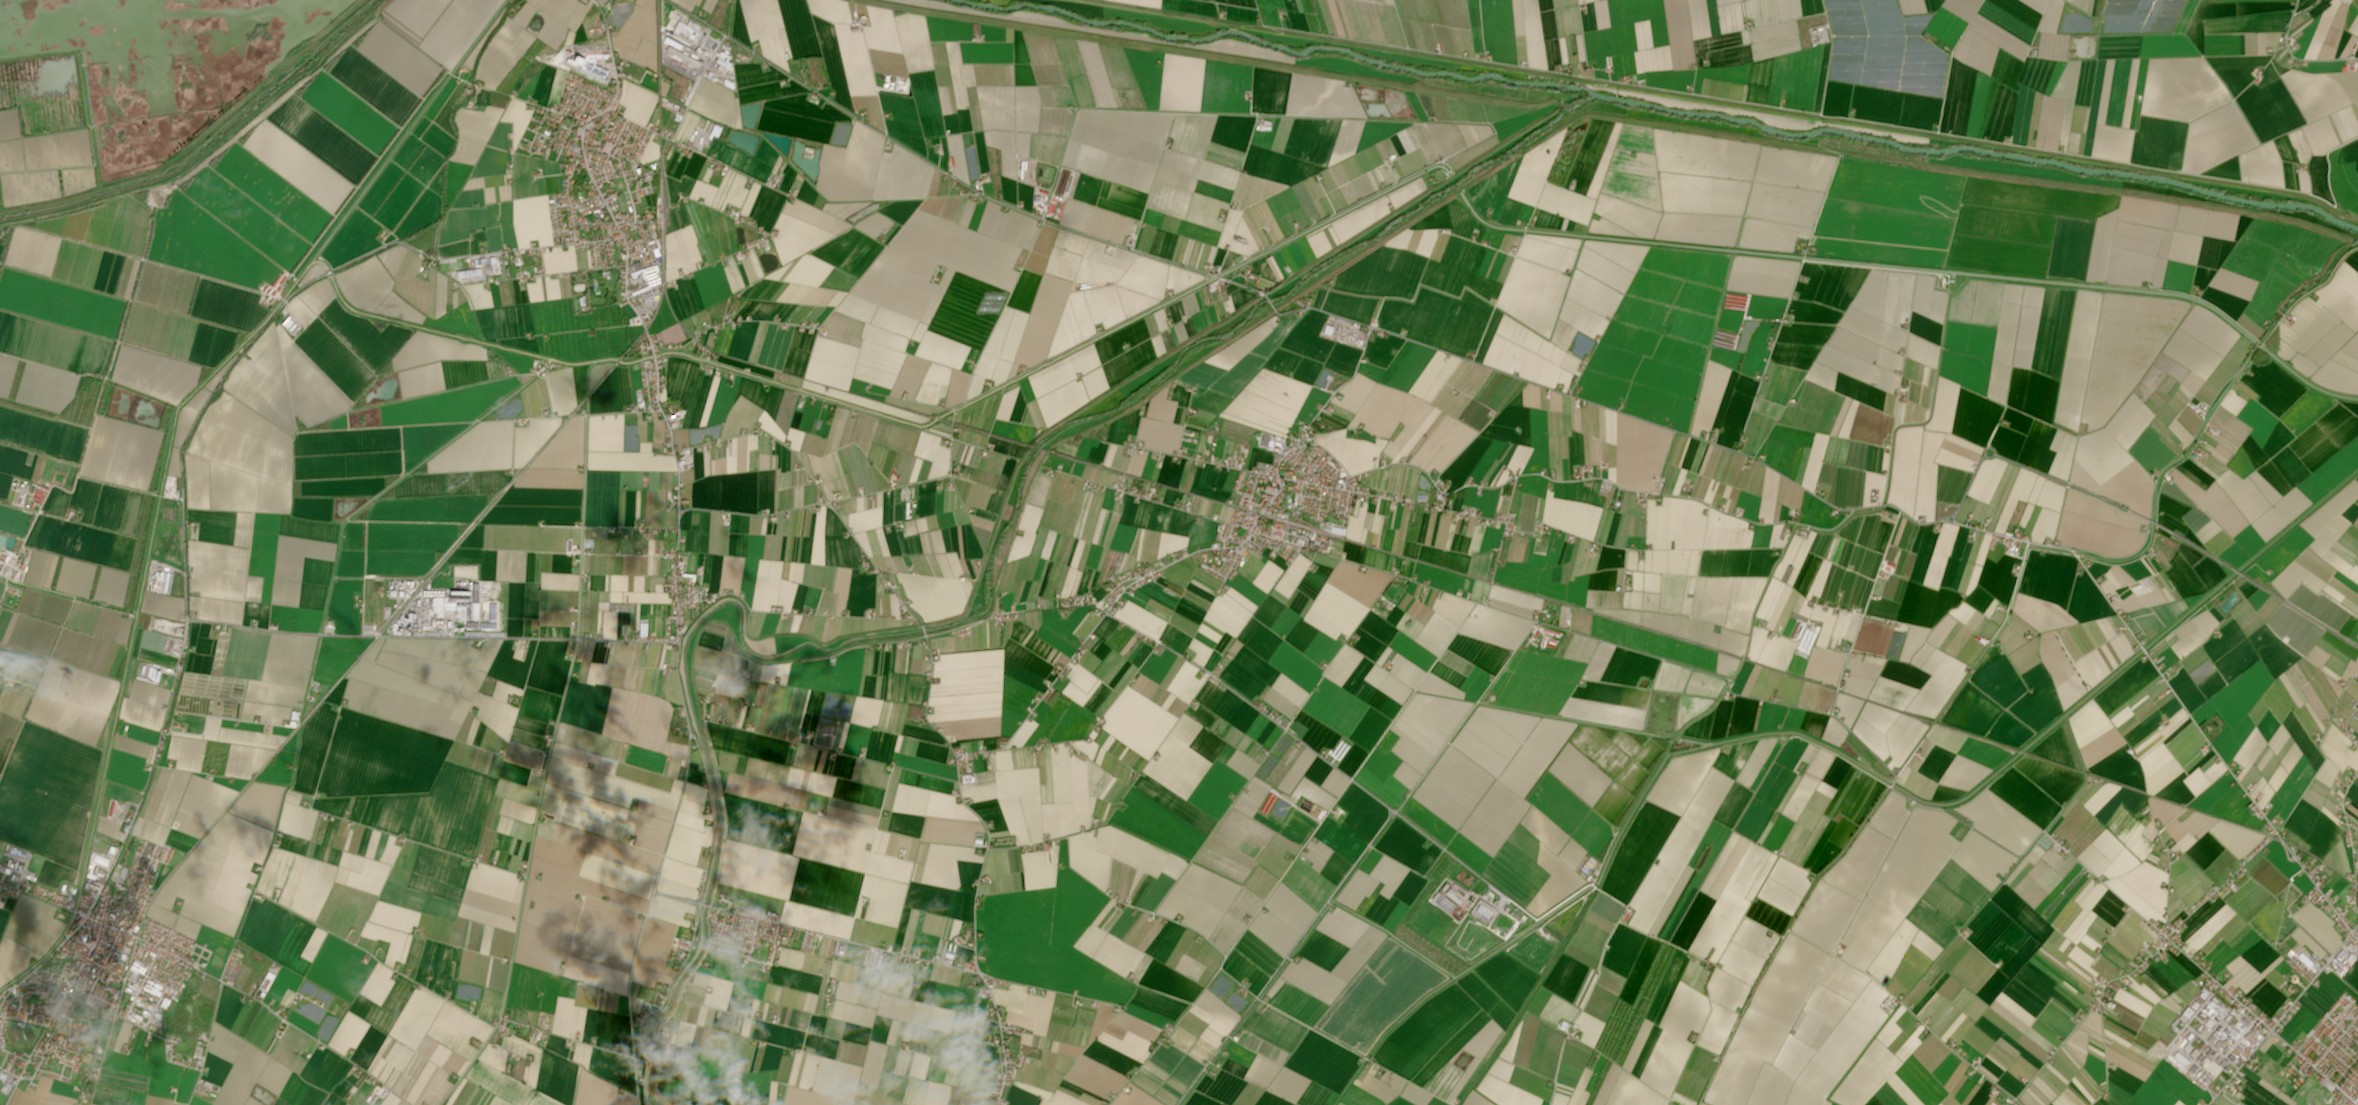
\includegraphics[width=\textwidth]{figures/2023-04-03-00_00_2023-04-03-23_59_Sentinel-2_L2A_True_color.jpg}
        \caption{Before-event true color image for Emilia-Romagna acquired on 3 April 2023.}
        \label{fig:emilia_truecolor_before}
    \end{subfigure}
    \hfill
    \begin{subfigure}[t]{0.49\textwidth}
        \centering
        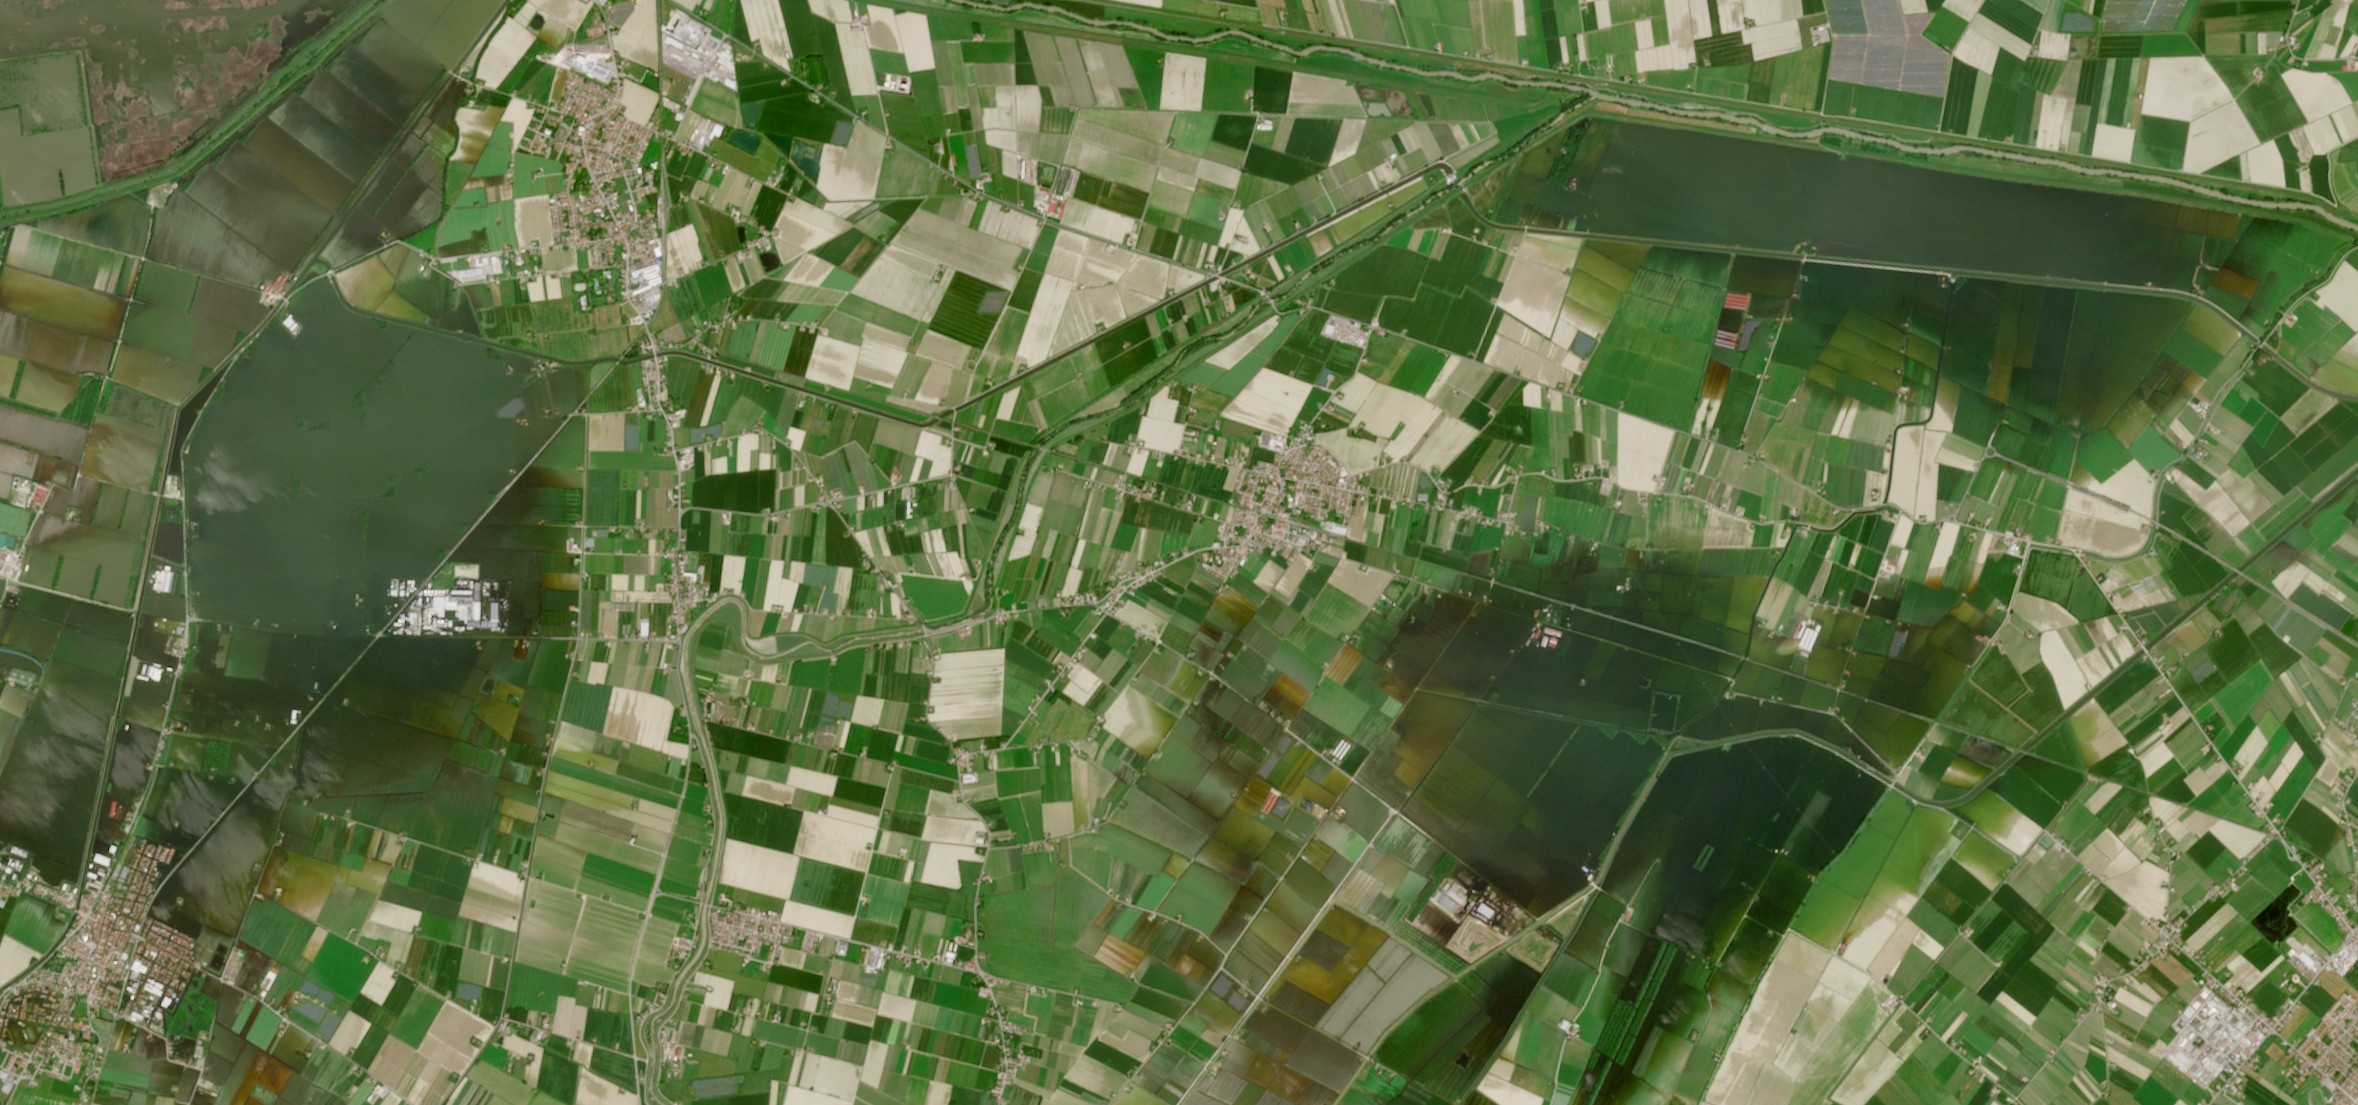
\includegraphics[width=\textwidth]{figures/2023-05-23-00_00_2023-05-23-23_59_Sentinel-2_L2A_True_color.jpg}
        \caption{After-event true color image for Emilia-Romagna acquired on 23 May 2023.}
        \label{fig:emilia_truecolor_after}
    \end{subfigure}
    \caption{Side-by-side comparison of Sentinel-2 true color imagery for the Emilia-Romagna flood case before and after the event. The comparison highlights the visible expansion of water-covered areas across the agricultural landscape.}
    \label{fig:emilia_truecolor_comparison}
\end{figure}

\begin{figure}[H]
    \centering
    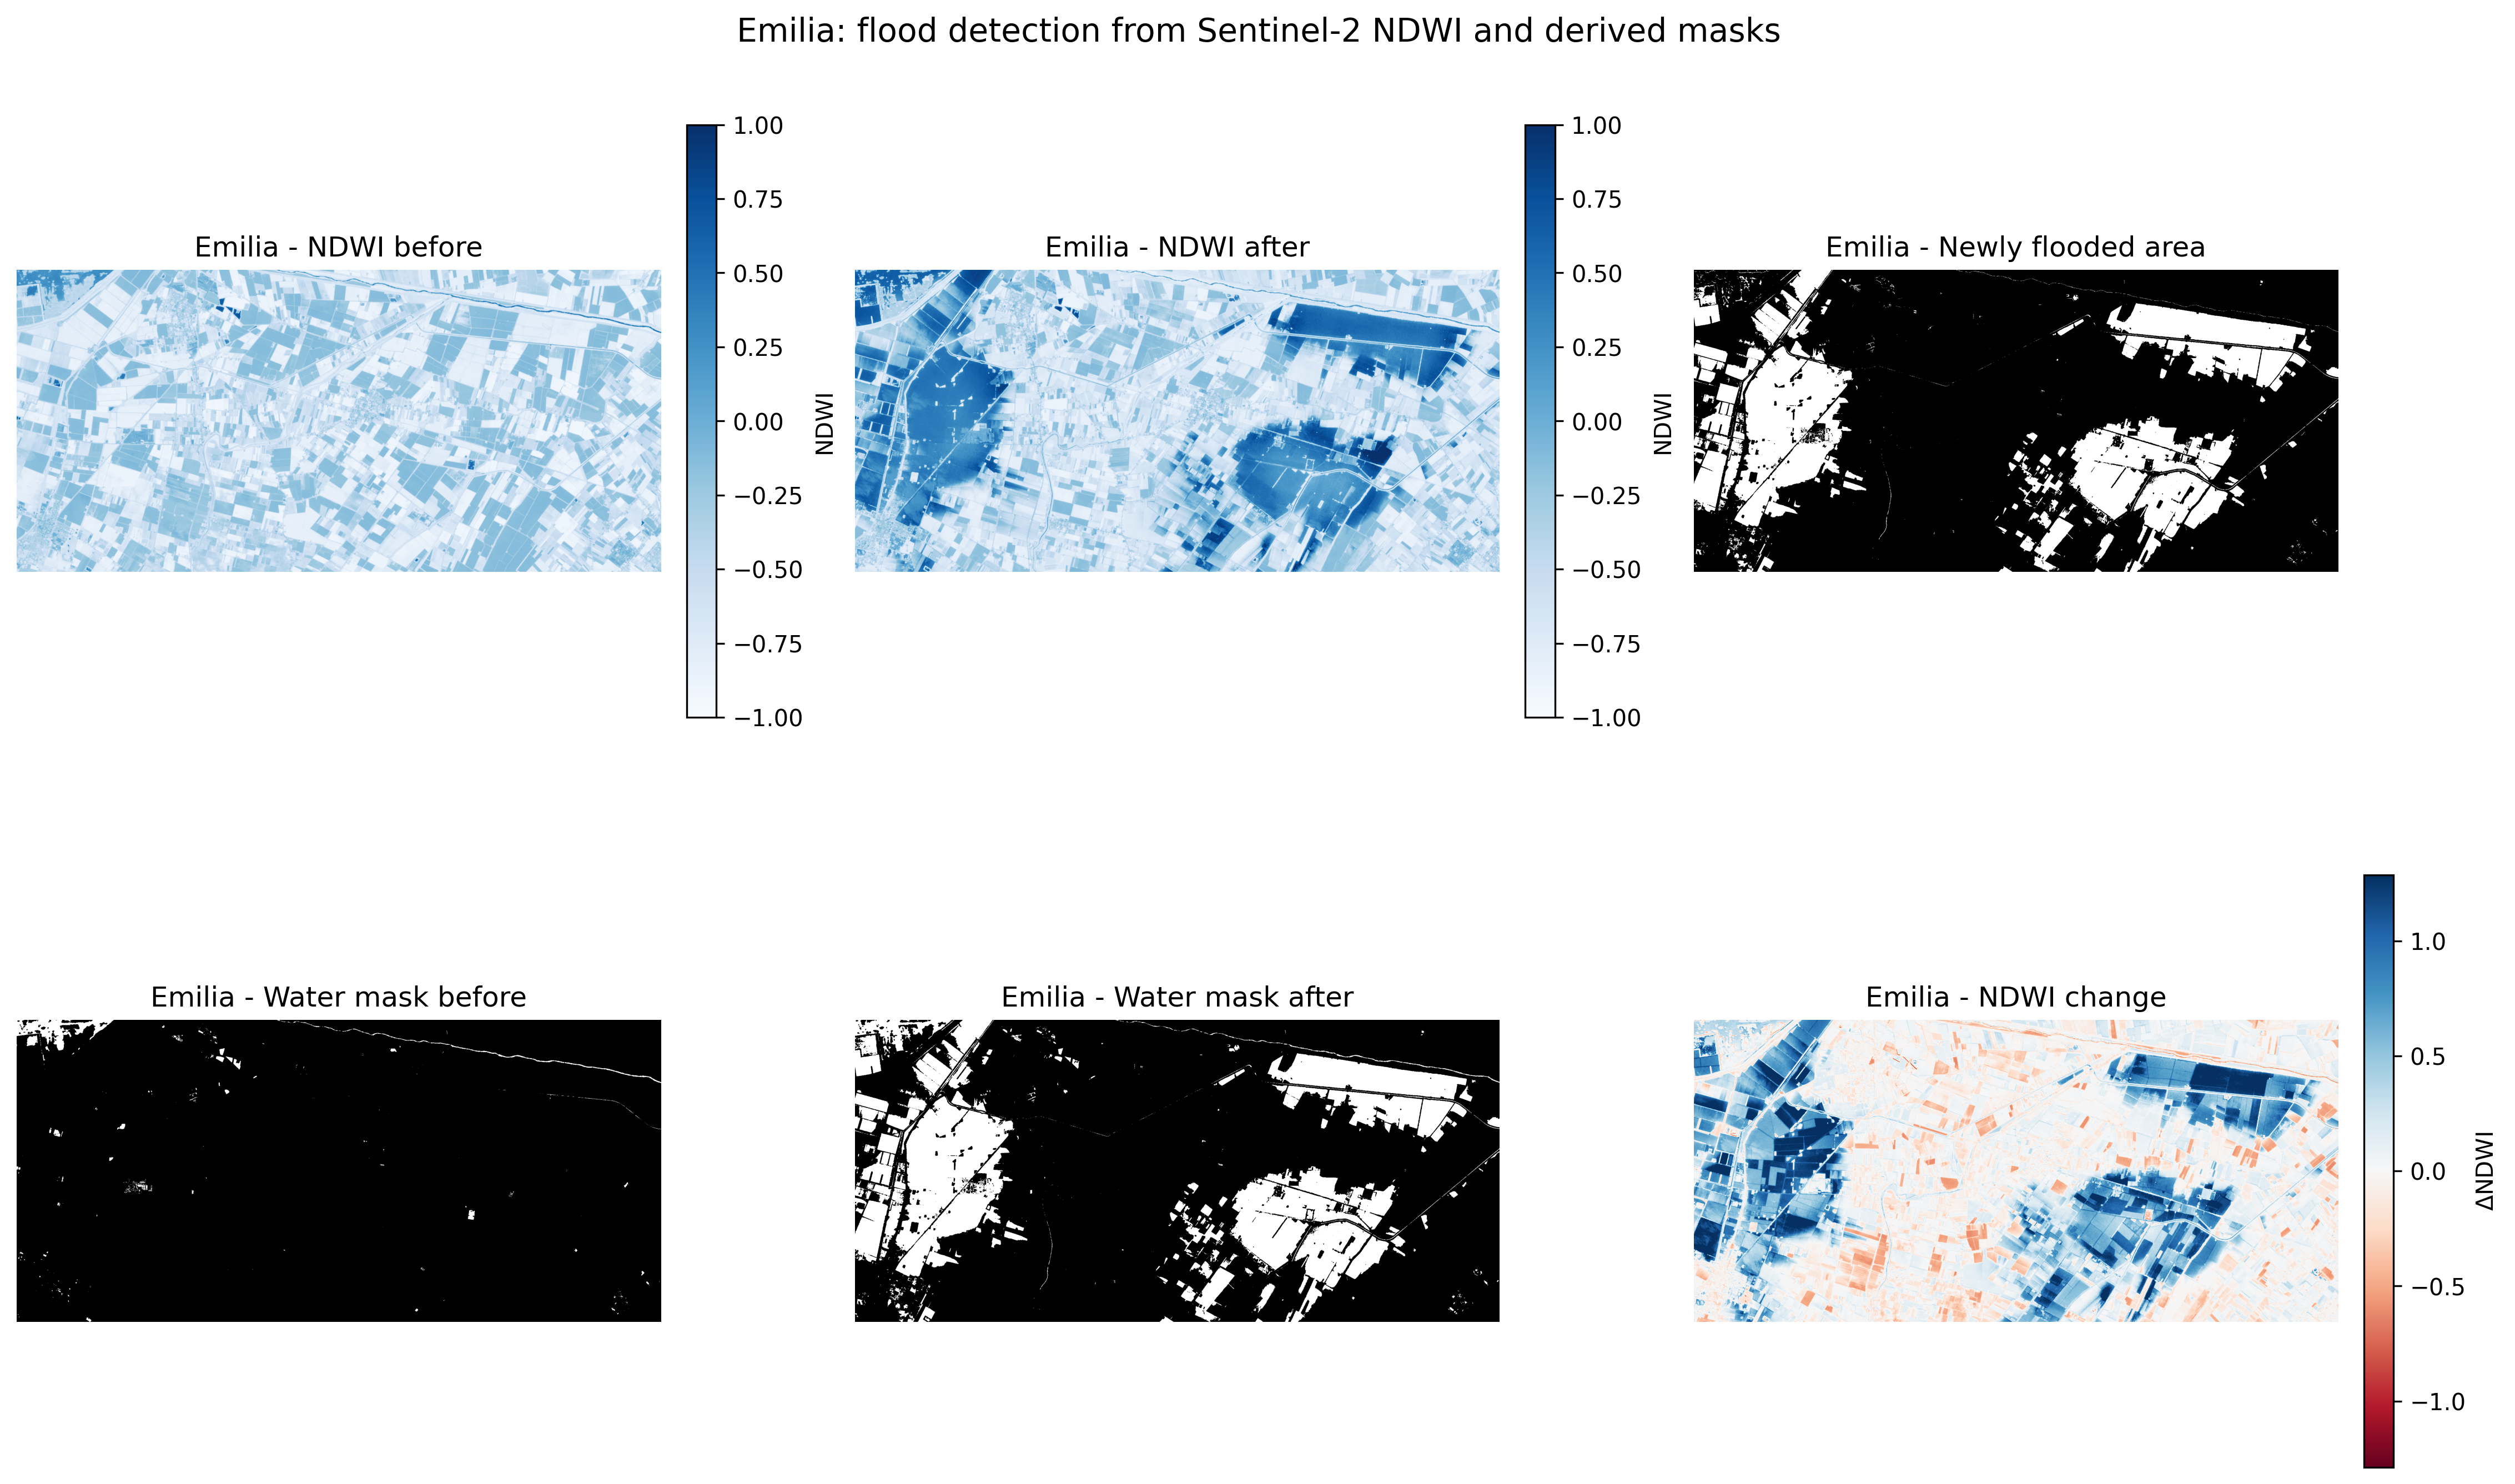
\includegraphics[width=\textwidth]{figures/Emilia_flood_report_figure.png}
    \caption{Flood detection results for Emilia-Romagna. The figure shows NDWI before and after the event, the newly flooded area mask, the water masks before and after the event, and the NDWI change map.}
    \label{fig:emilia_flood_report}
\end{figure}

\subsubsection{Wildfire Results}

\begin{table}[H]
\centering
\caption{Wildfire indicators derived from Sentinel-2 imagery}
\resizebox{\textwidth}{!}{
\begin{tabular}{lcccccc}
\toprule
Event & NDVI before & NDVI after & NDVI drop & dNBR & Veg loss (\%) & Burned area (\%) \\
\midrule
Greece & 0.4516 & 0.3257 & 0.1259 & 0.0453 & 21.0630 & 13.8515 \\
Serra da Estrela & 0.4751 & 0.3944 & 0.0807 & 0.1419 & 16.3626 & 17.4823 \\
Turkey & 0.3559 & 0.2871 & 0.0688 & -0.0763 & 14.1518 & 3.6802 \\
\bottomrule
\end{tabular}
}
\end{table}

The wildfire events show different levels of vegetation loss and burn severity. The Greece wildfire presents a strong vegetation loss and a large burned area, while the Serra da Estrela event shows a strong burn signal reflected in the dNBR value. The Turkey wildfire shows a smaller burned area, although vegetation loss is still detectable. Following we present the Turkey case.

\begin{figure}[H]
    \centering
    \begin{subfigure}[t]{0.49\textwidth}
        \centering
        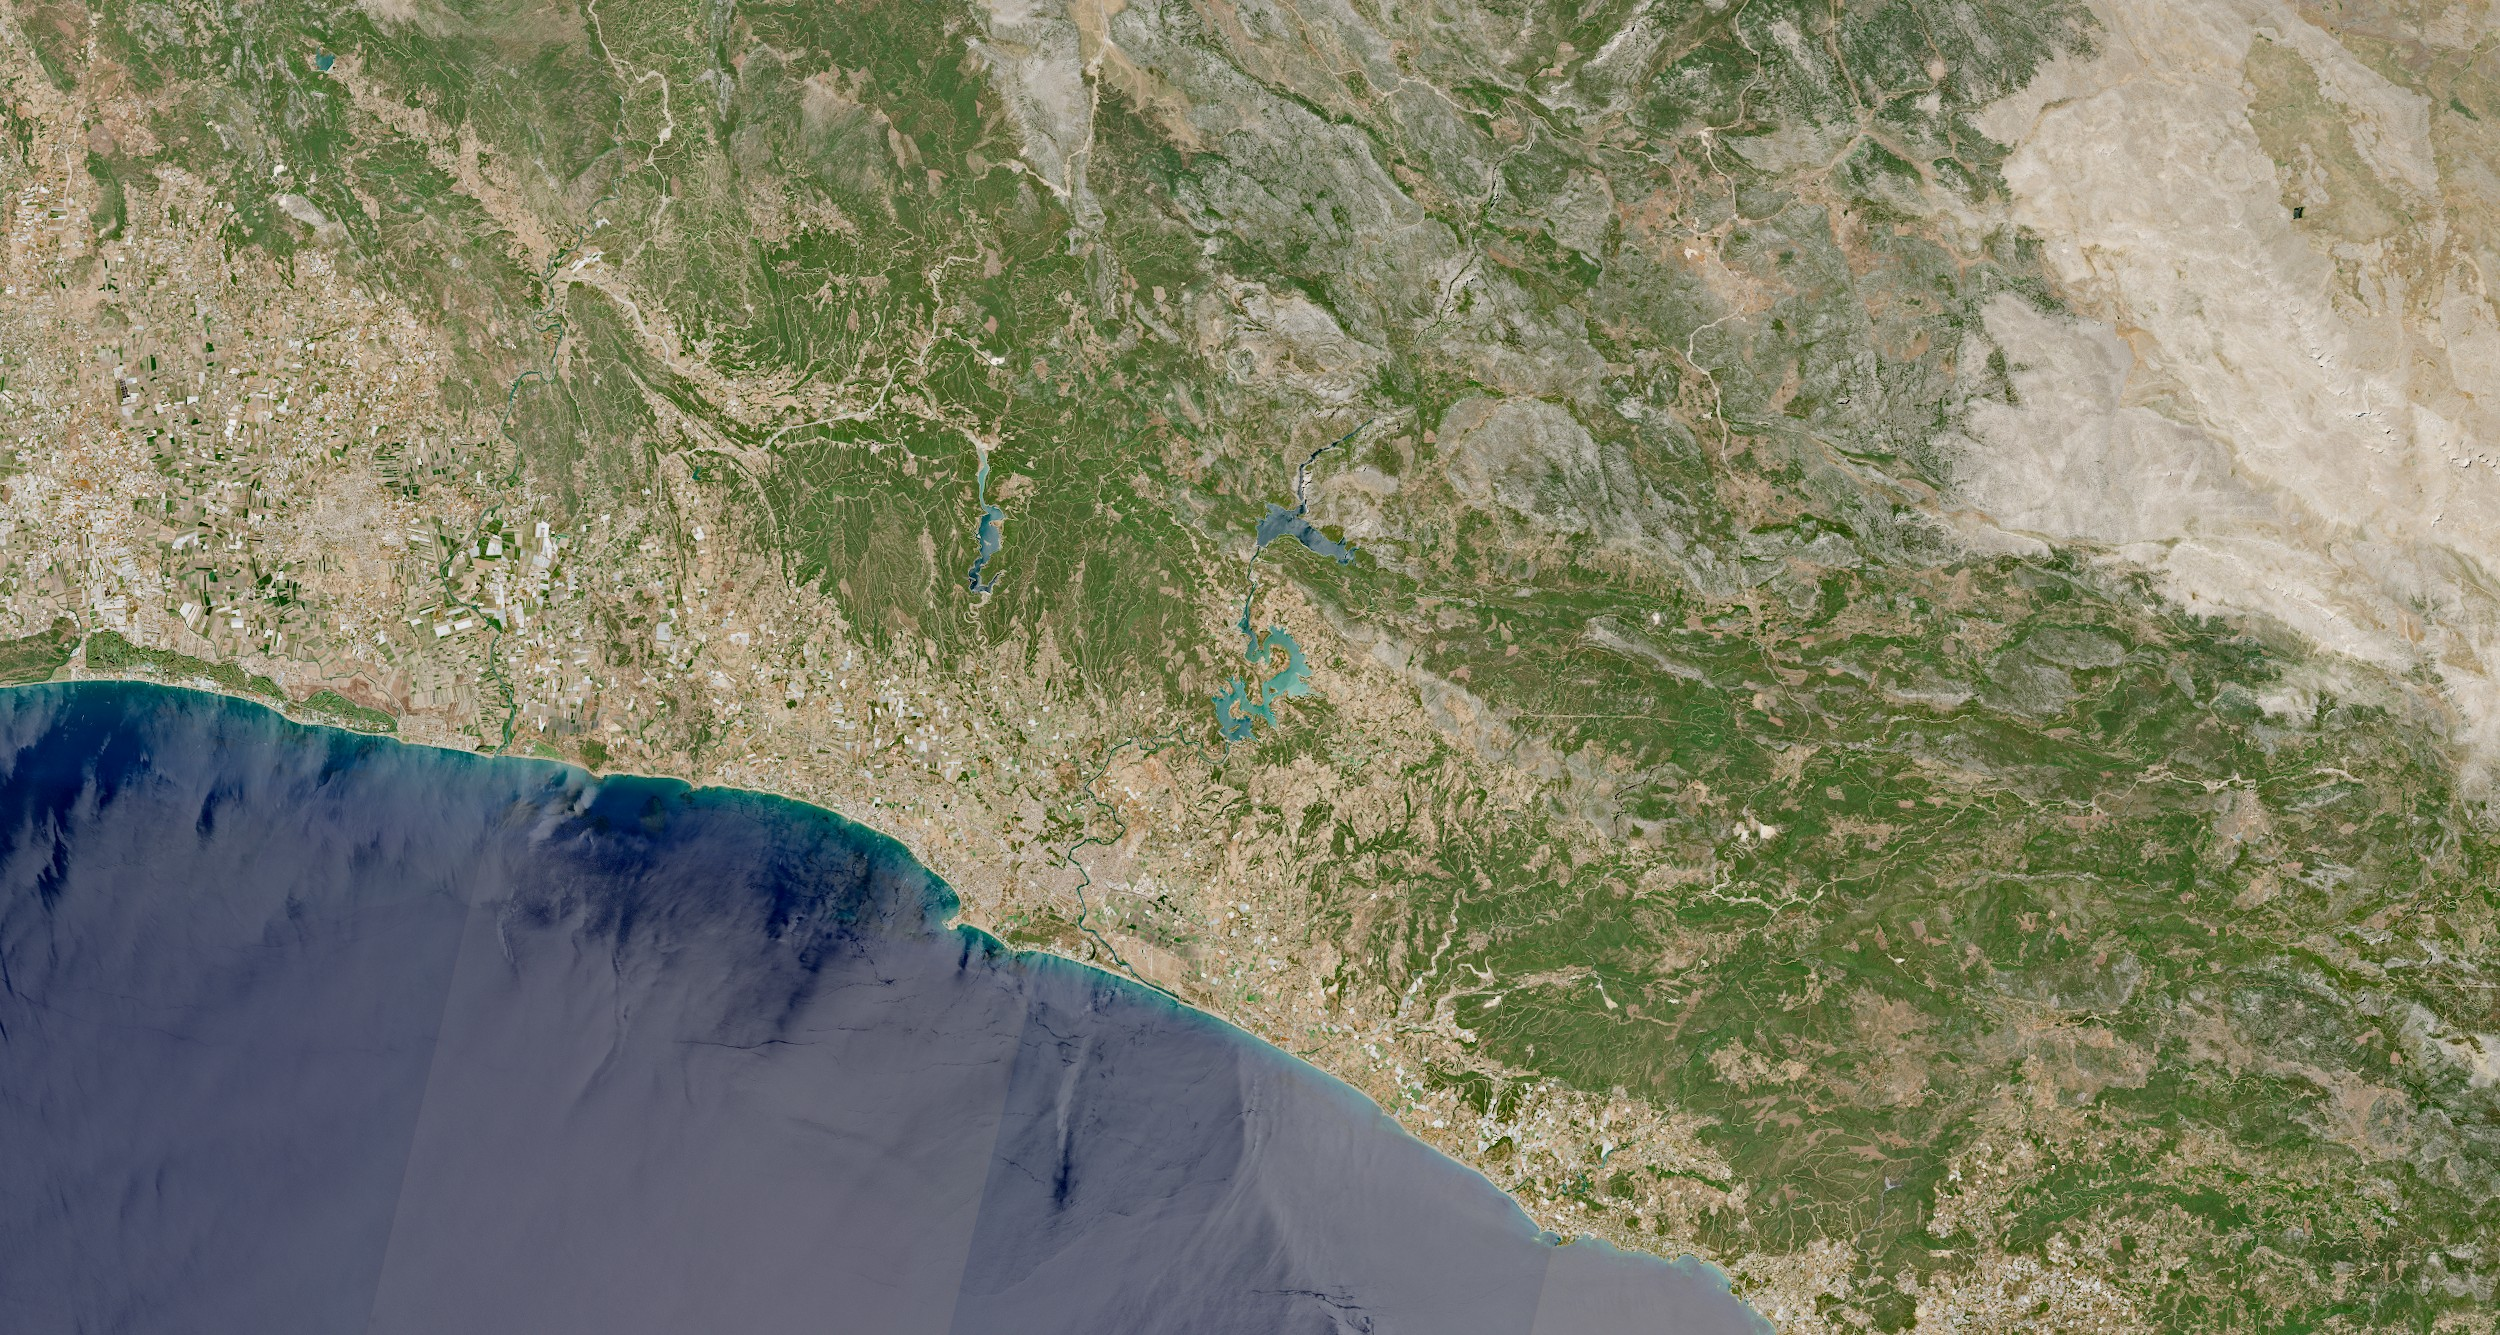
\includegraphics[width=\textwidth]{figures/2021-06-30-00_00_2021-06-30-23_59_Sentinel-2_L2A_True_color.jpg}
        \caption{Before-event true color image for the Turkey wildfire acquired on 30 June 2021.}
        \label{fig:turkey_truecolor_before}
    \end{subfigure}
    \hfill
    \begin{subfigure}[t]{0.49\textwidth}
        \centering
        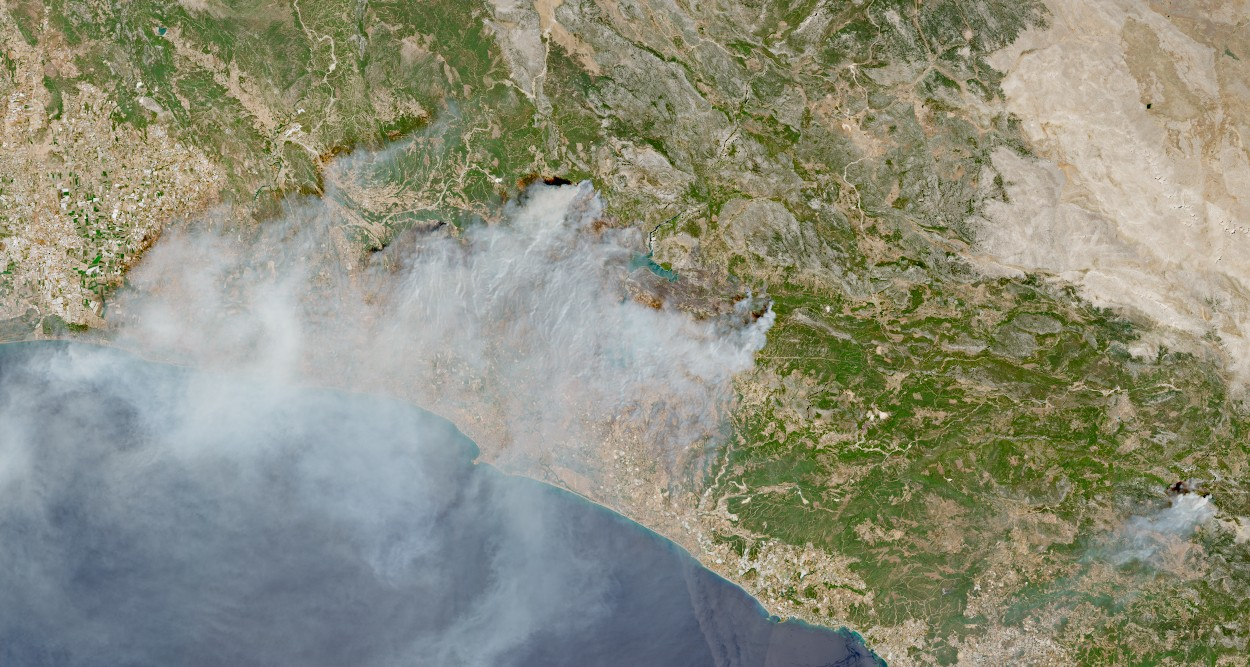
\includegraphics[width=\textwidth]{figures/2021-07-30-00_00_2021-07-30-23_59_Sentinel-2_L2A_True_color.jpg}
        \caption{After-event true color image for the Turkey wildfire acquired on 30 July 2021.}
        \label{fig:turkey_truecolor_after}
    \end{subfigure}
    \caption{Side-by-side comparison of Sentinel-2 true color imagery for the Turkey wildfire case before and after the event. The after-event image shows smoke and visibly altered surface conditions associated with the wildfire.}
    \label{fig:turkey_truecolor_comparison}
\end{figure}

\begin{figure}[H]
    \centering
    \includegraphics[width=\textwidth]{figures/Turkey_wildfire_report_figure.png}
    \caption{Wildfire detection results for Turkey. The figure shows NDVI before and after the event, dNBR, NBR before and after the event, and the derived burn mask.}
    \label{fig:turkey_wildfire}
\end{figure}

\end{document}